\section{Generation of a counterfactual explanation}
\subsection{generation by loss function}
CF explanation doesn't require to understand the internal work principle of a model, instead focusing on which kind of minimal perturbation in the data subject will leads to a different classification result. Therefore, the search of a an appropriate CF example is boiled down to an optimizing problem with at least two requirements: (1.) classified as the counter class, and (2.) still similar to the original data with only necessary modifications. \cite{watcher2017} has proposed the following formulation, which becomes the basis of the following research:
\begin{equation}\label{eq:watcher}
  \textbf{c}=\arg\min_{\textbf{c}}trgtloss(f(\textbf{c}),y)+d(\textbf{x,c})
\end{equation}
where \textbf{x} is the original data, y is the target data class, \textbf{c} is the generated counterfactual data, and f is the model so that f(\textbf{c}) is the new prediction of the model, i.e. the new class. The first part of the formula encourages a different class, while the second part penalizes large distances away from the original data.

To facilitate equation \ref{eq:watcher} one need to define it in detail, namely how to define "loss" and "distance", which has a significant impact on final results. Another main contribution of \cite{watcher2017} is to define distance as \emph{$L_1$} norm divided by MAD (median absolute deviation):
%统一字母代号: 
% K是特征,feature channel
% N是样本 instances
% D是什么?
% i 分类类别
\begin{equation}\label{eq:distOriginal}
  dist = \sum_{k=1}^{K}\frac{|\textbf{x-c}|}{MAD_k}
\end{equation}
where MAD is defined for every feature k over the whole points set P:
\begin{equation}\label{eq:MAD}
  MAD_k=median_{i\in P}(|{X_{i,k}}-median_{j\in P}(X_{j,k})|)
\end{equation}
The \emph{$L_1$} norm in equation \ref{eq:distMAD} prone to generate zero entries, which ensures a sparse optimizing result. Normalising the norm is important as well, otherwise big range data would have heavy weights. Here MAD turns out to outperform standard deviation, because it cooperates with \emph{$L_1$} norm better, and generates a even more sparse result.

Sometimes data may contain categorical features (e.g. occupation, gender\dots), it is counter-intuitive to define "distance" for these features. A simple matching distance is used here, where distance 1 is assigned to value changes and 0 if the value remains unchanged.
\begin{equation}\label{eq:distCate}
  dist\_cat(\textbf{c,x})=\sum_{k=1}^{K_{cat}}\mathbb{I}(c^k\neq x^k)
\end{equation}
Combining equation \ref{eq:distMAD} and \ref{eq:distCate} weighted by the number of continuous and categorical features, the most common used distance metric is shown as following:
\begin{equation}\label{distCombined}
  d(\textbf{x,c})=\frac{1}{K_{con}}\sum_{k=1}^{K_{con}}\frac{|\textbf{x-c}|}{MAD_k}
  +\frac{1}{K_{cat}}\sum_{k=1}^{K_{cat}}\mathbb{I}(\textbf c^k
  \neq \textbf x^k)
\end{equation}

Choosing an appropriate loss term for the target class is of equal importance. Without loss of generality, in this article we choose 0 as the original class label, and 1 for the desired label. Note that the prediction of the model f(\textbf{c}) is a continuous value between 0 and 1 for binary classification. One of the choices of the target loss term is the \emph{$L_2$} norm $(f(\textbf{c})-y)^2$. \cite{DiCE} argues that a valid counterfactual suffices if it bypasses the classification threshold of the model (typically 0.5), but the \emph{$L_2$} norm always prefer the extreme value 1. The underlying issue is that counterfactuals, unless predicted exactly as 1, still receives penalty even if it is classified correctly. A better choice is the hinge-loss:
\begin{equation}\label{eq:hingeloss}
  hinge\_trgtloss=\max(0,1-logit(f(\textbf{c})))
\end{equation}
\begin{figure}
  \centering
  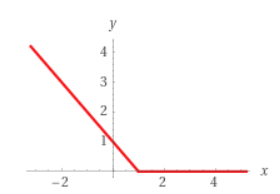
\includegraphics[]{hingeloss.PNG}
  \caption{the hinge loss penalize wrong classification heavily, correct one near the boundary slightly and has no effect above a certain threshold}\label{fig:hingeloss}
\end{figure}
where \emph{logit(f(\textbf{c}))} is the final activation before entering a sigmoid/softmax output layer. This loss function, however, requires internal logits of the model, therefore not available under a "black-box" situation.

So far the equations are derived for a binary classification problem, where a "why A not $\neg${A}" or "why A not B" question is raised. For n-ary classification, where the prediction output is a n-length vector, \cite{prototype} mentioned the following formula:
\begin{equation}\label{eq:lossPred}
  predloss=\max([f(\textbf{c})]_{i=i_0}-\max_{i\neq i_0}[f(\textbf{c})]_i),-\kappa)
\end{equation}
where $i_0=\arg\max f(\textbf{x})$ is the original data label, and $[f(\textbf{c})]_i$ is the i-th class prediction probability. This loss function gives a negative value if the predicted class is different than the original class, and $-\kappa < 0$ caps the negative value.

After fulfill the equation \ref{eq:distOriginal} in detail, it is already able to generate counterfactuals.
\subsubsection{add a diversity term}
As mentioned in the introduction, providing a diverse list of counterfactuals to choose from could be more helpful rather than one single "most feasible" solution. A valuable CF algorithm is able to generate multiple counter instances that are distinct from each other, but in a moderate way. The counterfactuals should still proximate the original input, rather than changing numerous features, or changing too fiercely. This is realized by adding a specific diversity loss term to the loss function. \cite{DiCE} proposed to use the determinant of a kernel matrix as the diversity metric for n counterfactuals:
\begin{equation}\label{eq:dpp}
  dpp\_diversity(\mathbf{c_1,\dots,c_n})=\det(\mathbf{K}),\ \mathbf{K}_{i,j}=\frac{1}{1+dist(\mathbf{c_i,c_j})}
\end{equation}
%TODO: DPP的数学特征?
This matrix is named after DPP (determinantal point processes), which is a widely adopted method in diversity constraint problems (e.g. diverse videos recommendation). An interesting mathematical property of this metric is its symmetric form with an all-one diagonal.
\subsubsection{add an interpretability term}
During the search of a CF example, it is equally important to demonstrate that the example is representable for the counter class, otherwise it is neither informative nor reasonable. For example, a user may want to change his occupation for better credits, but change the occupation to "professor" with educational background unchanged as "middle school" does not seem like a plausible answer. One trivial solution, as mentioned in the conclusion of \cite{bertossi2020asp}, is to abandon data generation, and only choose a closest case with the opposite label from a data bank. 

To handle with this issue, \cite{prototype} proposed a prototype loss term, to measure the distance from the generated CF to other CF classes in latent layer. For each CF class \emph{i}, the algorithm firstly picks out the N nearest neighbours of the input that are classified as \emph{i}, then feeds them through an encoder and averages the output as the prototype of this CF class.
\begin{equation}\label{eq:prototype}
  proto_i=\frac{1}{N}\sum_{n=1}^{N}\mathbf{ENC}(\mathbf{x_n^i})
\end{equation}
Among all prototypes, the closest one to the input is chosen as the "guidance" for optimization:
\begin{equation}\label{eq:closestProto}
  j = {\arg\min}_{i\neq f(\textbf{x})}||\mathbf{ENC}(\textbf{x})-proto_i||_2
\end{equation}
The prototype loss term is defined as following:
\begin{equation}\label{eq:protoloss}
  prtloss=||\mathbf{ENC}(\textbf{c})-proto_j||_2^2
\end{equation}
With the guidance of prototype, the perturbation is oriented to one chosen CF class rather than random search. The encoder used here could be any external known model, therefore requiring no internal information of the "black-box" model in question.  